%
%  nietzsche.five
%
%  Created by Mark Eli Kalderon on 2008-03-01.
%  Copyright (c) 2008 Mark Eli Kalderon. All rights reserved.
%
%  Beamer

% Definitions and macros
\newcommand{\change}{\textcolor{blue}{\textbf{CHANGE SLIDE}}}
\nwcommand\myauthor{Mark Eli Kalderon} 
\newcommand\mytitle{Introduction to Moral Philosophy}
\newcommand\mysubtitle{Nietzsche}
\newcommand\myinstitution{University College London}
\newcommand\myurl{http://markelikalderon.com/teaching}

% Packages specific to lecture notes
\mode<article>{
    \usepackage{palatino}
    \setjobnamebeamerversion{nietzsche.five.beamer}
}

% Packages specific to beamer presentation
\mode<presentation>{
    \usetheme{Darmstadt}
    \setbeamercovered{transparent}
    \pgfdeclareimage[height=0.5cm]{university-logo}{../../../graphics/logo_sml_blk}
    \logo{\pgfuseimage{university-logo}}
}

% Packages common to lecture notes and beamer presentation
\usepackage{pgf}
\usepackage{tikz}
\usepackage{hyperref}

\title{\mytitle}
\subtitle
{\mysubtitle}

\author{\myauthor\\
\url{\myurl}}
\institute{\myinstitution}

% \date[Short Occasion] % (optional)
% {Date / Occasion}

\begin{document}

\frame{\maketitle}

\change\ The title of the third essay, ``What is the significance of the ascetic idea'' is in one way misleading. As we have seen, for Nietzsche, things do not simply have significance or meaning, they are given it by a power that gains mastery over it. Given Nietzsche's interpretivism, the question ought to be posed as: ``What is the significance of the ascetic ideal for \ldots''---where what fills in the blank is the agency that has gained mastery over the ideal in some area of life or moment of history. Like the concepts of morality and punishment, there is no unique set of defining features associated with an ideal in virtue of which it is ascetic. We have distinct ascetic ideals associated with the artist, the philosopher, and, what is the real topic of the third essay, the Judaic priest. At best there is an overlapping pattern of resemblance in virtue of which each of these spearate ideals counts as ascetic. Like the concepts of morality and punishment, the concept of an ascetic ideal is a family of resemblance concept. Not strict definition can be given, where a strict definition is understood as providing non-trivial necessary and sufficient conditions since this ideal has participated in a long histry where different wills have gained mastery over it and those imposed different and not necessarily compatible interpretations and functions on this ideal. And the result is that at best there is a loose overlapping pattern of resemblance obtaining among all things that have so far been called an ascetic ideal.

Though no strict definition of an ascetic ideal can be given the rough idea is easy enough to state. An ideal is ascetic if involves foregoing certain pleasures in the interests of furthering something one deems to be more valuable. Consider then the significance of the ascetic ideal for the artist. If one is a painter one can't quite be drunk all the time if one is going to paint. A certain pleasure is foregone at some of the time in order to further some interest that the artist deems to be more valuable, namely, the production of his art. It is important to emphasize that this implementation of an ascetic ideal is the implementation of a prudential value. Given the artist's interests, the production of his art, it is important to disavow certain pleasure at least some of the time. Abstinence from drink is not a moral injunction that the artist observes nor is it universally observed; rather, the artist abstains from drink to the degree to which it is necessary in order to further his art. This distinction, between the prudential understanding of an ascetic ideal and a moralizing understanding of it as imposed by a priestly will is important in what follows. Nietzsche never criticizes ascetic ideals in and of themselves. Indeed he commends asceticism as a form of prudence when it is in the service of furthering a certain kind of life.

I have already mentioned the case of the artist as an example of this. Nietzsche also believes that asceticism as it occurs in philosophical practice is also of prudential value. Nietzsche writes:
\begin{quote}
    Every animal---therefore \emph{la bete philosophe}, too---instinctively strives for an optimum of favorable conditions under which it ca expend all its strength and achieve its maximal feeling of power; every animal abhors, just as instinctively and with a subtlety of discernment that is higher than all reason every kind of intrusion or hindrance that obstructs or could obstruct this path to the optimum \ldots\ What then is the meaning of the ascetic ideal in the case of a philosopher? My answer is---you will have guessed it long ago: the philosopher sees in it an optimum condition for the highest and boldest spirituality and smiles---he does not deny existence, he rather affirms his existence and only his existence, and this to the point to which he is not far from harboring the impious wish: Let the world perish, but let there be philosophy, the philosopher, me!
\end{quote}
Like the artist, the philosopher sees in the ascetic ideal the natural conditions under which his form of life can flourish. So in the case of both the artist and the philosopher a certain kind of asceticism is the natural condition under which a certain form of creativity can flourish---certain minimal forms of self-constraint can be willed by artists ad philosophers as preconditions of their creativity, of their will to power.

Given how Nietzsche evaluates or determines the value of values, it should be clear that this kind of prudential asceticism is beyond criticism. Recall the fundamental Aristotelian insight that drives Nietzsche's moral philosophy---a value is positively or negatively valuable only to the extent to which it promotes or hinders human flourishing. Insofar as a certain kind of asceticism forms the natural conditions for the flourishing of a certain kind of life, such asceticism is beyond reproach. To repeat, Nietzsche has no quarrel with asceticism per se. In its prudential variety, it is obviously valuable for certain forms of life, the artist, the philosopher, etc. What Nietzsche criticizes is not the ascetic ideal insofar as it forms the optimum conditions for the flourishing of a certain form of life, rather, his target is the ascetic ideal as understood by the religiously serious Christian. \change

\begin{frame}<presentation>[label=slide1]
    \frametitle{Asceticism}
        \begin{columns}
            \begin{column}{3cm}
                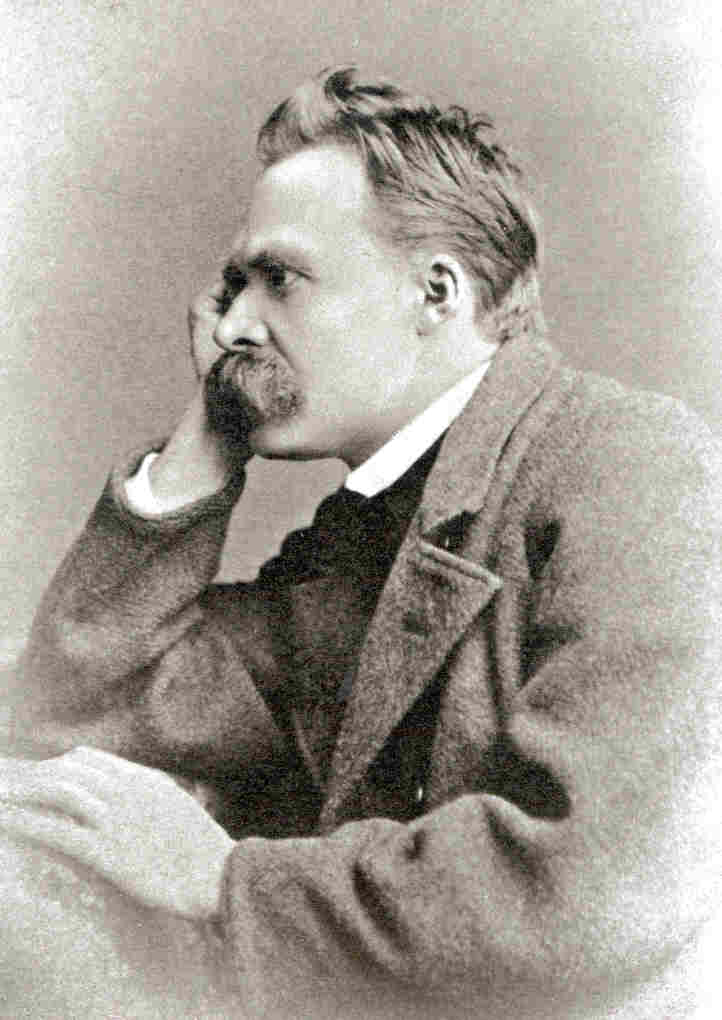
\includegraphics[height=4cm]{../../../graphics/nietzsche.jpg}
            \end{column}
            \begin{column}{7cm}
                If one wants to lead a certain kind of life then certain minimal measures of rational self-control appropriate to that life ought to be observed
            \end{column}
        \end{columns}
\end{frame}

So the question with which we must begin is what is the significance of the ascetic ideal for the religiously serious Christian. Since Nietzsche believes that this significance was imposed by a priestly will, ultimately St. Paul's, our question is what is the meaning of the ascetic ideal for the Judaic priest? Nietzsche's provisional answer to this question will take the form of an antimony. We might call it the \emph{antimony of priestly asceticism}:
\begin{quote}
    The function of asceticism for the priest is to deny life itself. But since the pries is part of life, priestly asceticism is an apparent contradiction---it represents the opposition of life against life.
\end{quote}

We will spend a fair amount of time considering what Nietzsche means by this. But what I want to emphasize at the outset is the provisional nature of his answer. In particular, like the Kantian antimonies, Nietzsche believes that the paradox or contradiction is only apparent. Recall the antimony of style. The function of style is to foster both understanding and misunderstanding. The contradiction involved in this literary paradox was only seen to be merely apparent once the function of style was more deeply understood. Namely there is an important discriminatory function of style. Literary style functions so as the text will only be understood by its intended audience. Once this discriminatory function of style is discerned, then the paradox is resolved. Nietzsche believes that all such apparent contradictions have a resolution---that there is always a naturalistic resolution for such apparent paradoxes. And so to with the antimony of priestly asceticism. Insofar as the meaning of the ascetic ideal for the pries is to oppose life to life, its meaning has not been fully understood. That is why this answer to the question what is the meaning of the ascetic ideal for the priest is at best a provisional answer. So our first task is to understand why Nietzsche believes that Christian asceticism is fundamentally opposed to life. Our second task is to see how Nietzsche resolves this apparent paradox. Our third task is to answer the question, ``What is the significance of the ascetic ideal for Nietzsche?'' That is, given Nietzsche's account of its meaning or significance, how does he propose to get mastery of these ascetic ideals and impose upon them his own new function and meaning. Just by way of preview, it is notable that in one of his unpublished notes, Nietzsche writes that he wishes to ``renaturalize asceticism'' with the goal of strengthening and not negating the will. Strengthening the will and enhancing life seem to be more or less the same thing here, so it seems that Nietzsche's overall intention in the \emph{Genealogy} is to take over the traditional way of life associated with the ascetic ideal and renaturalize its asceticism in the interests of the enhancement and affirmation of life. More on this as we proceed. \change

\begin{frame}<presentation>[label=slide2]
    \frametitle{Antimony of Priestly Asceticism}
        \begin{columns}
            \begin{column}{3cm}
                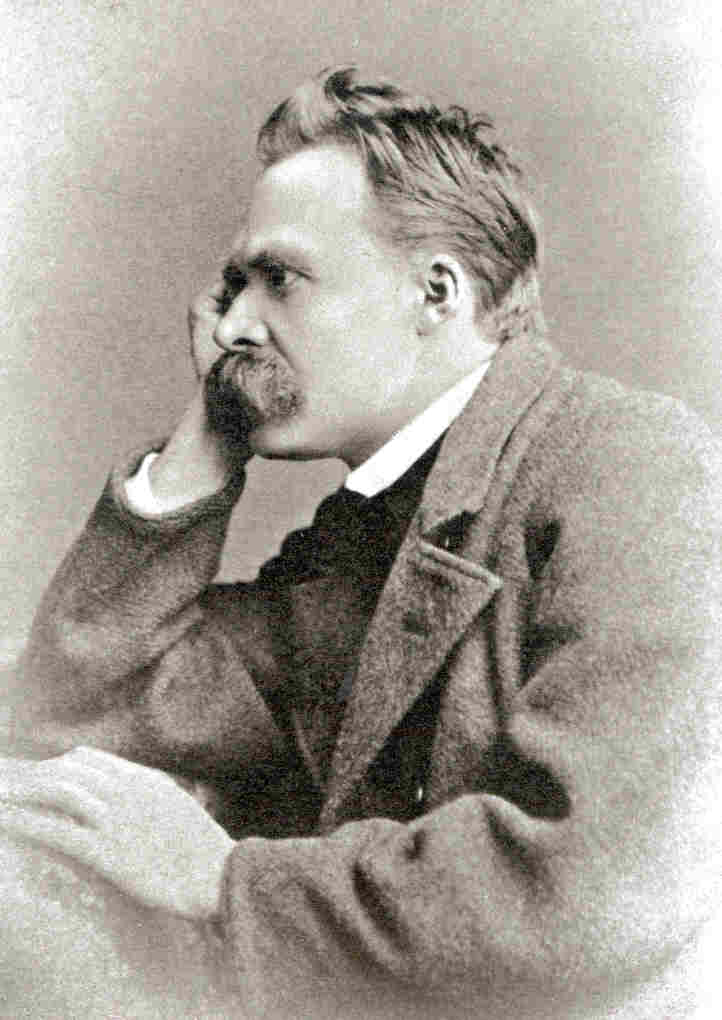
\includegraphics[height=4cm]{../../../graphics/nietzsche.jpg}
            \end{column}
            \begin{column}{7cm}
                The function of asceticism for the priest is to deny life itself. But since the pries is part of life, priestly asceticism is an apparent contradiction---it represents the opposition of life against life.
            \end{column}
        \end{columns}
\end{frame}

Why does Nietzsche believe that Christian asceticism is fundamentally hostile to life itself? To see this we must once again return to our genealogy. Recall the genealogical tree that I gave you. The topic of the third essay concerns the bottom right hand quadrant of that tree:

\begin{center}
    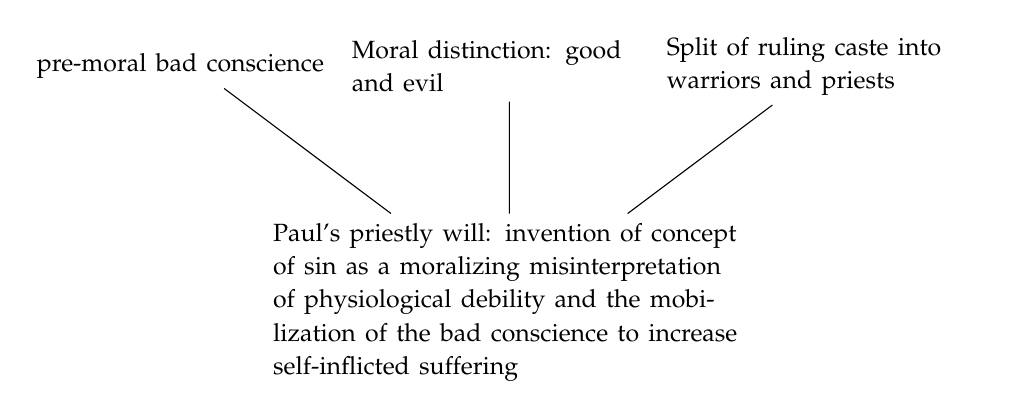
\begin{tikzpicture}
        \tikzstyle{level 1}=[sibling distance=4cm]
        \node[text width=6cm] {\small{Paul's priestly will: invention of concept of sin as a moralizing misinterpretation of physiological debility and the mobilization of the bad conscience to increase self-inflicted suffering}} [grow'=up]
            [level distance=3cm]
            child {node[text width=4cm] {\small{pre-moral bad conscience}}}
            child {node[text width=4cm] {\small{Moral distinction: good and evil}}}
            child {node[text width=4cm] {\small{Split of ruling caste into warriors and priests}}};
    \end{tikzpicture}
\end{center}

So far we have been discussed the mechanism involved in the historical production of the pre-moral bad conscience and how the basic moral distinction between good and evil was established by the ressentiment of the slaves. We have yet to discuss, however, what Nietzsche sees as an internal conflict in aristocratic society, that is, the conflict between the military and priestly subcastes of the nobility. Nietzsche's discussion of this occurs in sections 6 and 7 of the first essay of the \emph{Genealogy}. Recall what was driving Nietzsche in the first essay was the great wealth of philological evidence that suggests that terms originally denoting political superiority resolve over time into terms denoting moral or spiritual superiority. In section 6 of the first essay, Nietzsche deals with a putative counterexample to what I have been calling his \emph{fundamental philological hypothesis}---that our moral language originates in terms denoting political stations. What about the moral and spiritual distinction between the pure and the impure? Within the Christian tradition these terms have obvious moral and spiritual significance, but it is hard to see how they originally had any political significance. Given the empirical nature of Nietzsche's argument of this essay, this is an important objection and one that must be dealt with if he is to make the far reaching conclusions that he does on the basis of philological evidence. How does Nietzsche deal with this putative counterexample to his fundamental philological hypothesis? \change

\begin{frame}<presentation>[label=slide3]
    \frametitle{The Sub-Genealogy}
        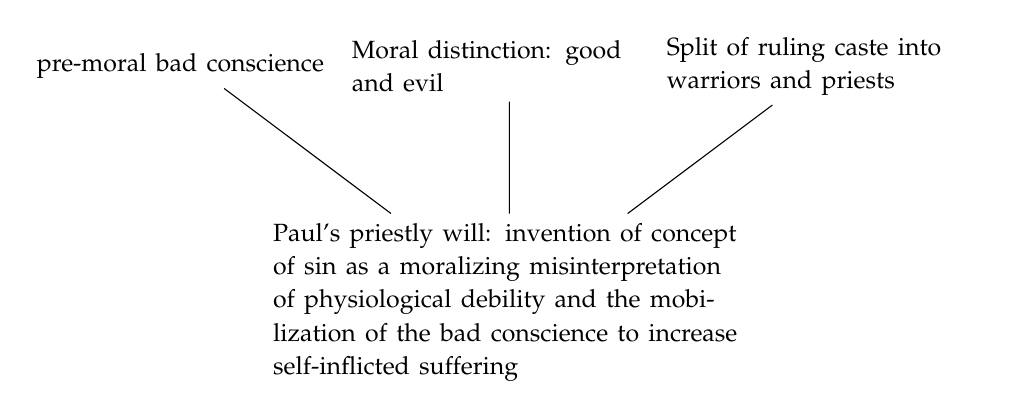
\begin{tikzpicture}
            \tikzstyle{level 1}=[sibling distance=4cm]
            \node[text width=6cm] {\small{Paul's priestly will: invention of concept of sin as a moralizing misinterpretation of physiological debility and the mobilization of the bad conscience to increase self-inflicted suffering}} [grow'=up]
                [level distance=3cm]
                child {node[text width=4cm] {\small{pre-moral bad conscience}}}
                child {node[text width=4cm] {\small{Moral distinction: good and evil}}}
                child {node[text width=4cm] {\small{Split of ruling caste into warriors and priests}}};
        \end{tikzpicture}
\end{frame}

Nietzsche's response comes in two parts. First he points out that originally talk of purity and impurity had nor moral or spiritual significance. Nietzsche writes:
\begin{quote}
    One should be warned, moreover, against taking these concepts ``pure'' and ``impure'' too ponderously or broadly, not to say symbolically: all the concepts of ancient man were rather at first incredibly uncouth, coarse, external, narrow, straightforward, and altogether unsymbolical in meaning to a degree that we can scarcely conceive. The pure one is from the beginning merely a man who washes himself, who forbids himself certain foods that produce skin ailments, who does not sleep with dirty women of the lower strata, who has an aversion to blood---no more, hardly more.
\end{quote}

Originally, then, the concepts of pure and impure do not have the moral and spiritual significance that they will come to have in the Christian tradition. Purity in its Christian moralized sense is in effect a metaphor, whereas originally talk of purity was meant quite literally. It only designated certain practices of cleanliness more or less broadly conceived. The fundamental point that Nietzsche is making here is that talk of purity and impurity was only invested with moral or spiritual significance as the result of subsequent historical developments. Originally these terms were devoid of moral or spiritual content.

That they eventually come to have such content is due in part to an internal conflict between the military and priestly subscastes of the nobility. The priests came to differentiate themselves and affirm this difference by designating themselves in terms that referred specifically to ritual purity. The priests made a point of engaging in the practice of ritual purity, in the abstinence from certain foods, the avoidance of menstruating women, and so on in order to positively affirm their difference from the military faction of the nobility. This is Nietzsche's second point, terms used to designate ritual purity were in fact invested with political significance; they were definitive of a certain subcaste of the nobility, namely, the priestly subcaste. The opposition between the pure and the impure is thus not a genuine counterexample to Nietzsche's fundamental philological hypothesis. Nietzsche in effect concedes that it is not obvious that ritual purity designated a political station, but suggests that a careful review of the historical record will reveal otherwise. Purity originally had no moral or spiritual significance, and came to denote a political station, namely, that of the priestly subcaste of the nobility, when this subcaste came to use terms denoting ritual purity to differentiate themselves from the military faction of the aristocracy.

Talk of purity and impurity were only invested with a specifically moral content as the result of the role the priestly subcaste played in the slave revolt in morality. Nietzsche suggests that the division of the nobility into these two subcastes was an uneasy one, and that there developed between the priestly and military factions of the nobility a relation of jealous opposition. Nietzsche in effect hypothesizes an internal power struggle within the nobility. The priests lost out in this power struggle and were dominated by the military faction of the nobility. The priests subsequently threw in with and actively participated in the slave revolt in morality.

There is some philological evidence for this. Unlike the terms denoting the military faction of the nobility, which in the noble mode of evaluation became good and in the moral mode of evaluation became evil, terms originally designating ritual purity which were used by the priests to designate their political station did not in the moral mode of evaluation come to be evil rather; rather, they were associated with the good as it figures in the moral mode of evaluation. Why were these terms that were used to designate the priestly caste of the nobility not associated with evil once the slave revolt in morality was complete? Precisely because the priests sided with the slaves and actively participated in the salve revolt. They were prompted to do so as a result of their losing out in an internal power struggle within the nobility.

Already, then, in the first essay, we can see the origins of Christian asceticism. That Christian morality is an ascetic morality is in large part due to the fact that the priests made common cause with the slaves in the slave revolt of morality. Notice that terms denoting ritual purity in terms of which the priests differentiated themselves from the military faction of the nobility all have to do with abstinence---abstaining from certain foods, abstaining from menstruating women, etc. Imbuing talk of ritual purity with moral significance was in effect the erection of the ascetic ideal as it functionsin Christian morality.

How did the priests erect the ascetic ideal? They managed to do this by using two very different forces, namely the \emph{ressentiment} that animated the salve revolt in morality and the bad conscience. It is worth emphasizing their difference. \emph{Ressentiment} is essentially directed outward---it is the hostile reaction to some external force that has dominated, that has won out in a struggle for power. The bad conscience is always directed inward---it is the result of internalizing aggression that could not be externally discharged. The priests' art was, in effect, to use these two very different forces to organize and animate Christian asceticism. \change

\begin{frame}<presentation>[label=slide4]
    \frametitle{Purity}
        \begin{itemize}
            \item Purity originally designates only certain practices of cleanliness
            \item Purity is then invested with political significance when the priests distinguish themselves from the military subcaste of the nobility in terms of ritual purity
            \item Purity only receives a moral interpretation when the priests make common cause with the slaves in the slave revolt of morality
        \end{itemize}
\end{frame}

Earlier, I distinguished, in a preliminary fashion, a prudential variety of asceticism from the moralized asceticism of Christianity. In its prudential form, asceticism is nothing more than a minimal kind of rational self-control required to promote the flourishing of a certain kind of life. In its prudential variety asceticism is merely of instrumental value. As a matter of prudence, asceticism is in effect a hypothetical imperative: if one is to engage in a certain form of life, then at a minimum one must abstain from certain things. The claims of prudential asceticism are thus conditional. Moreover, not all goods are abstained from and those that are abstained from are not necessarily abstained from all of the time. In its prudential variety, Nietzsche has no problem with asceticism. It is only the moralizing interpretation foisted upon ascetic practices by the priests that Nietzsche seeks to oppose. Indeed, Nietzsche's own positive ethical views themselves constitute a kind of asceticism---a renaturalized asceticism. So the third essay should not be read as condemning all asceticism, only the ascetic morality of Christianity.

How different Christian moral asceticism is from the prudential asceticism that Nietzsche commends. Whereas the claims of prudential asceticism are conditional, the claims of a moralized asceticism are unconditional: one must, unconditionally, abstain from certain pleasures. Prudential ascetics need not dogmatically insist that other forms of life will benefit if they too forego the goods and pleasures that they deny themselves. The moral ascetic, however, does insist upon just this: the claims of moral asceticism are unconditional and \emph{universal}---they apply equally to all and are not relativized to a specific form of living. And whereas prudential asceticism only demands that one forego those goods and pleasures that would hinder the flourishing of a certain form of life, moral asceticism is not that discriminating. Rather than insisting that certain pleasures must be avoid in order to secure others that one values more highly, moral asceticism insists that one avoids \emph{all} pleasure.

There are three salient differences, then, between prudential and moral asceticism:
\begin{itemize}
    \item The claims of prudential asceticism are \emph{conditional} whereas the claims of moralized asceticism are \emph{unconditional}
    \item The claims of prudential asceticism apply \emph{only at certain times and place and to certain forms of life} whereas the claims of moralized asceticism are \emph{universal} in scope
    \item Prudential asceticism counsels only the avoidance of \emph{certain goods and pleasures} whereas moral asceticism counsels the avoidance of \emph{all earthly goods and pleasures}
\end{itemize}

Despite these striking differences, moral asceticism retains something of the rationale that motivates prudential asceticism. Nietzsche writes:
\begin{quote}
    The idea at issue here is the valuation the ascetic priest places on our life; he juxtaposes it (along with what pertains to it: nature, world, the whole sphere of becoming and transitoriness) with a quite a different mode of existence which it opposes and excludes, less it turns against itself, deny itself: in that case, the case of ascetic life, life counts as a bridge to that other mode of existence.
\end{quote}
The ascetic priest maintains that in the course of our earthly existence we must deny ourselves the pleasures that life affords in order to secure our heavenly reward. In propounding the fiction of an afterlife, the ascetic priest can resuscitate the rationale motivating prudential asceticism: one abstains from earthly goods in order to secure other goods, one's heavenly reward, that one values more highly. After all, what is mere riches compared to eternal bliss! But in propounding this fiction of an otherworldly existence, the ascetic priest and the moral asceticism he advocates is denying or devaluing our earthly existence. If, however, one maintains with Nietzsche that this earthly life is the only life we have, then one can only maintain that devaluation or denial of our earthly existence is nothing more than the devaluation or denial of life itself. From a naturalistic perspective, this is a strange predicament. After all, the priest and the moral asceticism that he propounds are both part of life. How then can be life be against life? Mark Hallis once put this point nicely in a song: ``You can't go against nature since going against nature is part of nature too''.

\begin{frame}<presentation>[label=slide5]
    \frametitle{Two Varieties of Asceticism}
        \begin{itemize}
            \item The claims of prudential asceticism are \emph{conditional} whereas the claims of moralized asceticism are \emph{unconditional}
            \item The claims of prudential asceticism apply \emph{only at certain times and place and to certain forms of life} whereas the claims of moralized asceticism are \emph{universal} in scope
            \item Prudential asceticism counsels only the avoidance of \emph{certain goods and pleasures} whereas moral asceticism counsels the avoidance of \emph{all earthly goods and pleasures}
        \end{itemize}
\end{frame}

This is what I called the antimony of priestly asceticism. If one insists, as Nietzsche does, on offering naturalistic accounts of everything, the mere existence of a form of life that turns itself against nature is a very serious problem, for this mode of life mist be accounted for by the same naturalistic mechanism that explain everything else. But then it appears that the ascetic life, which must be a natural phenomena like everything else:
\begin{quote}
    is itself a contradiction; here rules ressentiment without equal, that of an insatiable instinct and will to power that wants to become master not over something in life but over life itself, over its most profound, powerful, and basic conditions \ldots\ All this is to the highest degree paradoxical: we stand before a discord that wants to be discordant, that enjoys itself in this suffering and even grows more self-confident and triumphant the more its own presupposition, its physiological capacity for life decreases.
\end{quote}
This paradox, like the Kantian antinomies, is only apparent. That is why Nietzsche insists that such an interpretation is at best a provisional interpretation of moral asceticism. Nietzsche believes that apparently unnatural conditions are always in the final analysis means for accomplishing natural ends. What then ins the function of moral asceticism, if it isn't to deny life itself.

Remarkably, despite his deep aversion to it, Nietzsche ascribes to moral asceticism a function similar to that which he ascribed to Greek tragedy in his first book, \emph{The Birth of Tragedy}: tragedy and art generally apepars to draw people away from life, even to depict utter failure, only to show that life is worth living nonetheless. The ascetic priest is not only a physician and shepherd but in a very real sense a kind of artist, an artist in feelings of guilt. The ascetic priest denies life and turns against it, only to seduce his flock into continuing to live. Nietzsche writes:
\begin{quote}
    Such a self-contradiction that the ascetic priest appears to present, life against life, is physiologically considered and not merely psychologically, a simple absurdity. It can only be apparent. Let us replace it with a brief formulation of the facts of the matter: the ascetic ideal springs from the protective instinct of a degenerating life which tries by all means to sustain itself and to fight for its existence.
\end{quote}

What is the nature of the sickness that afflicts the degenerating life that moral asceticism seeks to preserve. Here we must confront a question first raised int eh second essay, namely the problem of suffering, The Nietzsche notes that there is a tendency in European culture to see in the existence of suffering an argument against life. One manifestation of this tendency is the problem of evil. The problem of evil uses the existence of suffering to argue that our belief in God is unjustified. But Nietzsche makes a rather astute observation as to hwy this tendency is ultimately unguided. Suffering itself, even if widespread and prolonged and terrible may be endured. What the human animal cannot endure is \emph{senseless suffering}---suffering without reason. The problem posed by suffering is not its existence but its apparent \emph{senselessness}. The sickness that the ascetic priest seeks to curve is a kind of social malaise that Nietzsche describes as the nausea and the pity of man. The social malaise is just the meaninglessness of suffering. The art of the ascetic priest is to invent an interpretation for this suffering to give it a meaning and thus allow the weak to endure it where they might have otherwise been tempted to do away with themselves.

The sickness, the malaise, that the ascetic priest seeks to cure is the senselessness of suffering thus allowing the weak to endure. Before we see how the ascetic priest constructs an interpretation of suffering from the raw materials of guilt and resentment, let's first inquire as to why the weak suffer. Nietzsche often imagines in a naive and sometimes crude way that the cause of this social malaise is straightforwardly physiological. Thus he speaks of the intestinal morbidity that typically afflicts priests or that the great nausea at man is quite literally a form of indigestion. It is hard to take this aspect of his view seriously. But we ought to take seriously the phenomena he describes as an illness: the pervasiveness of misery. The world for Nietzsche is full of people who are incapable of accomplishing what they hope to accomplish, people who want in vain to be brave, generous, strong, perhaps even cruel, or at least notorious in some way---people want to, but cannot, leave their mark on history. The weak suffer because they are too weak to realize their ambitions, to positively manifest their will to power.

What is horrible about physical or psychological suffering in Nietzsche's eyes is not the suffering itself, horrible as it may be. This, he believes, may be tolerated; it can even be persued if a reason exists for it, if it is a means to further achievement. The most repellent feature of human misery is just the fact that there is no reason for it. Since senseless misery forces the question why should one undergo it at all, it is crucial to offer an interpretation for it that explains and even justifies it (since if there is no reason to undergo the misery of one's daily life then suicide or self-destruction seems the only available option). The great achievement of the ascetic priest is that he explains suffering and that this explanation appeals to a guilty agent that is susceptible to suffering. In this way he supplies a cause, someone who is responsible for suffering, and also an object on whom those who suffer can vent their affects and so deaden by means of a violent emotion a tormenting secret pain that is becoming unendurable. But the ascetics interpretation involves on further essential twist. Recall the reactive nature of the lambs whose motto is you are evil and therefore I am good. Resentment prevails among the suffering as well. As Nietzsche writes:
\begin{quote}
    I suffer someone must be to blame for it---thus thinks every sickly sheep. But its shepherd, the ascetic priest, says ``Quite so, my sheep! Someone must be to blame for it; but you yourself are this someone you are alone to blame for it---you alone are to blame for yourself.''
\end{quote}

\section*{Summary}

\end{document}
